\chapter{Implementation}
This chapter discusses the implementation details of the proposed mobile application. First, the \gls{har} stages will be discussed. That includes the data gathering process from the project participants as well as data prepossessing and training of the kNN classifier. Next, the self-management system will be discussed followed by the specifics of the mobile application itself such as database and overall system design implementation.

\section{HAR System}
In order for the system to take actions such as notifying the user for a prolonged periods of inactivity or sending a notification when a \gls{pa} goal is achieved, the application needs to recognise human activities (i.e. walking and running). Implementation of the \gls{har} system will be discussed bellow.

    \subsection{Data Collection}
    One of the key stages in the development process of a typical supervised (online) \gls{har} system is the data collection stage. A labelled dataset is needed in order to train a model (or also called classifier). The produced model can classify an "unseen" (or unlabelled) data to a specific activity (i.e. walking or being static).
    
    \subsubsection*{Setting and project participants}
    The data needed to train the model in this work was collected from 3 fellow students in a controlled environment. Each one of the project participants was equipped with a device running partially implemented \textit{"Active Minutes"} application (e.g. only the \textit{"Data Collection screen"} see \ref{fig:data-collection-screen-design}). Before performing the data collection process, the participants had to, first, select the activity they will perform from a list of activities and then press the Start button on the application's UI in order to start the data collection process. The location of the device during the recording was chosen to be the front pants pocket. This location has been found to be the optimal position for \gls{har} (see \ref{section:non-commercial-har-systems}). All of the participants recorded 3 minutes of each one of the following activities: \textit{walking}, \textit{running}, \textit{cycling} and \textit{static}. To avoid any unwanted information during the recording stage, the first and the last 7 seconds of each activity was removed since it contained noise information such as the linear acceleration taking place when the device was put in and pulled out of participants pockets. That was pragmatically done and no direct human intervention was needed to further filter the data.
    
    \subsubsection*{Recorded data}
    \label{subsubsection:recorded_data}
    When all of the required data was collected, it was converted into a WEKA ARFF file format by pressing the "EXPORT" button on the Data Collection screen. The ARFF file was stored on the device's external memory (e.g. SD card). A sample of the produced ARFF file can be seen in Listing \ref{weka-arff-code}. A dataset containing ~720 labelled data points (or a total of ~36 minutes of data) was produced as a result of the data collection process. 
    
    The device used to collect the data was \textit{OnePlus One} equipped with low-power high performance 3-axes accelerometer \footnote{\url{http://www.st.com/en/mems-and-sensors/lis3dh.html}}. As for the sampling frequency (SF) of the sensor, the Android Operating system provides a total of four different sampling frequencies for reading the accelerometer sensor, namely \textit{NORMAL: 5 Hz}, \textit{UI: 16 Hz}, \textit{GAME: 50 Hz}, and \textit{FASTEST}. The latter has been chosen for the SF of the built-in accelerometer as it has produced good results in \citet[3-5]{lee2016}. According to the Google's documentation \textit{FASTEST} SF depends on the hardware of the device \citep{googlesensormanager2017}. In this case, the SF was \textbf{115} Hz. 
    
    \subsection{Training the kNN classifier}
    The exported ARFF Weka file (see section \ref{subsubsection:recorded_data}) is then bundled into the application itself by transferring the collected data straight into the \textit{Assets} directory of the mobile application. That allows for "shipping" the application with the collected training dataset. The \gls{knn} classifier is then trained and serialised when the \textit{onCreate} method of the \textit{Application} is called. This method is only called once during the life of the application \citep{googleapplication2017}.
    
    \subsubsection*{Accuracy}
    The ARFF Weka file (dataset) was tested externally on a PC to find the optimal \gls{knn} parameters such as the number of neighbours the classifier should consider before making a class prediction as well as whether to perform a cross validation of the data. The testing was done using the PC version of WEKA \footnote{\url{http://www.cs.waikato.ac.nz/ml/weka/}} Machine Learning application. After performing thorough testing, the default parameters of the \gls{knn} classifier performed the the best reaching accuracy of \textit{83.7\%} for dataset containing 763 data points. The performance for the trained model can be seen in table \ref{table:4_class_confusion_matrix}. 

    \begin{table}[ht]
    \centering
    \begin{tabular}{ |c|c|c|c||c| } 
     \hline
     a & b & c & d & classified as\\
     \hline \hline
     140 & 4 & 2 & 33 & a = walking \\
     57 & 112& 0 & 10 & b = running \\
     0 & 1 & 218 & 0 & c = static \\
     5 & 1 & 11 & 169 & d = cycling \\
     \hline
    \end{tabular}
    \caption{4 classes Confusion Matrix}
    \label{table:4_class_confusion_matrix}
    \end{table}

According to the confusion matrix in the table above, data points of class "running" has been incorrectly classified 57 times as class "walking" and 10 times as class "cycling". However, for the implementation purposes of the proposed application that performance of the model is still acceptable because even though the classifier has been designed to distinguish between 4 classes, only 2 classes are taken into account, namely "static" and "active" (including "walking", "running" and "cycling") on a programming level. Feature versions of the application may utilise the "active" classes to show a more detailed information to the user such as how much time the user has spend walking or running throughout the day.

To demonstrate the actual accuracy of the model taking account only those 2 classes, the original dataset has been modified so that only 2 classes are present - static and active. The confusion matrix after training the model(again the same \gls{knn} classifier with default parameters) can be seen in table \ref{table:2_class_confusion_matrix}. The actual accuracy of the classifier reaches 98.1\% since only 14 data points has been incorrectly classified.

    \begin{table}[ht]
    \centering
    \begin{tabular}{ |c|c|c| } 
     \hline
     a & b & classified as\\
     \hline \hline
      531 & 13 & a = active\\
      1 & 218 & b = static\\
     \hline
    \end{tabular}
    \caption{2 classes Confusion Matrix}
    \label{table:2_class_confusion_matrix}
    \end{table}
    
    \subsection{HAR System Implementation}
    The basic architecture of the \gls{har} system integrated into the application has been informed by \citet[149]{labrador2013}. For example, classes such as \textit{Point}, \textit{TimeSeries}, \textit{TimeWindow}, \textit{FeatureSet} and \textit{FeatureExtractor} form the core of the \gls{har} system. Simplified diagram of the \gls{har} system can be seen in figure \ref{fig:har_system_impl_class_diagram}. A brief discussion on the main responsibilities of the above-mentioned classes will is presented bellow.
    
    \begin{figure}[ht]
        \centering
        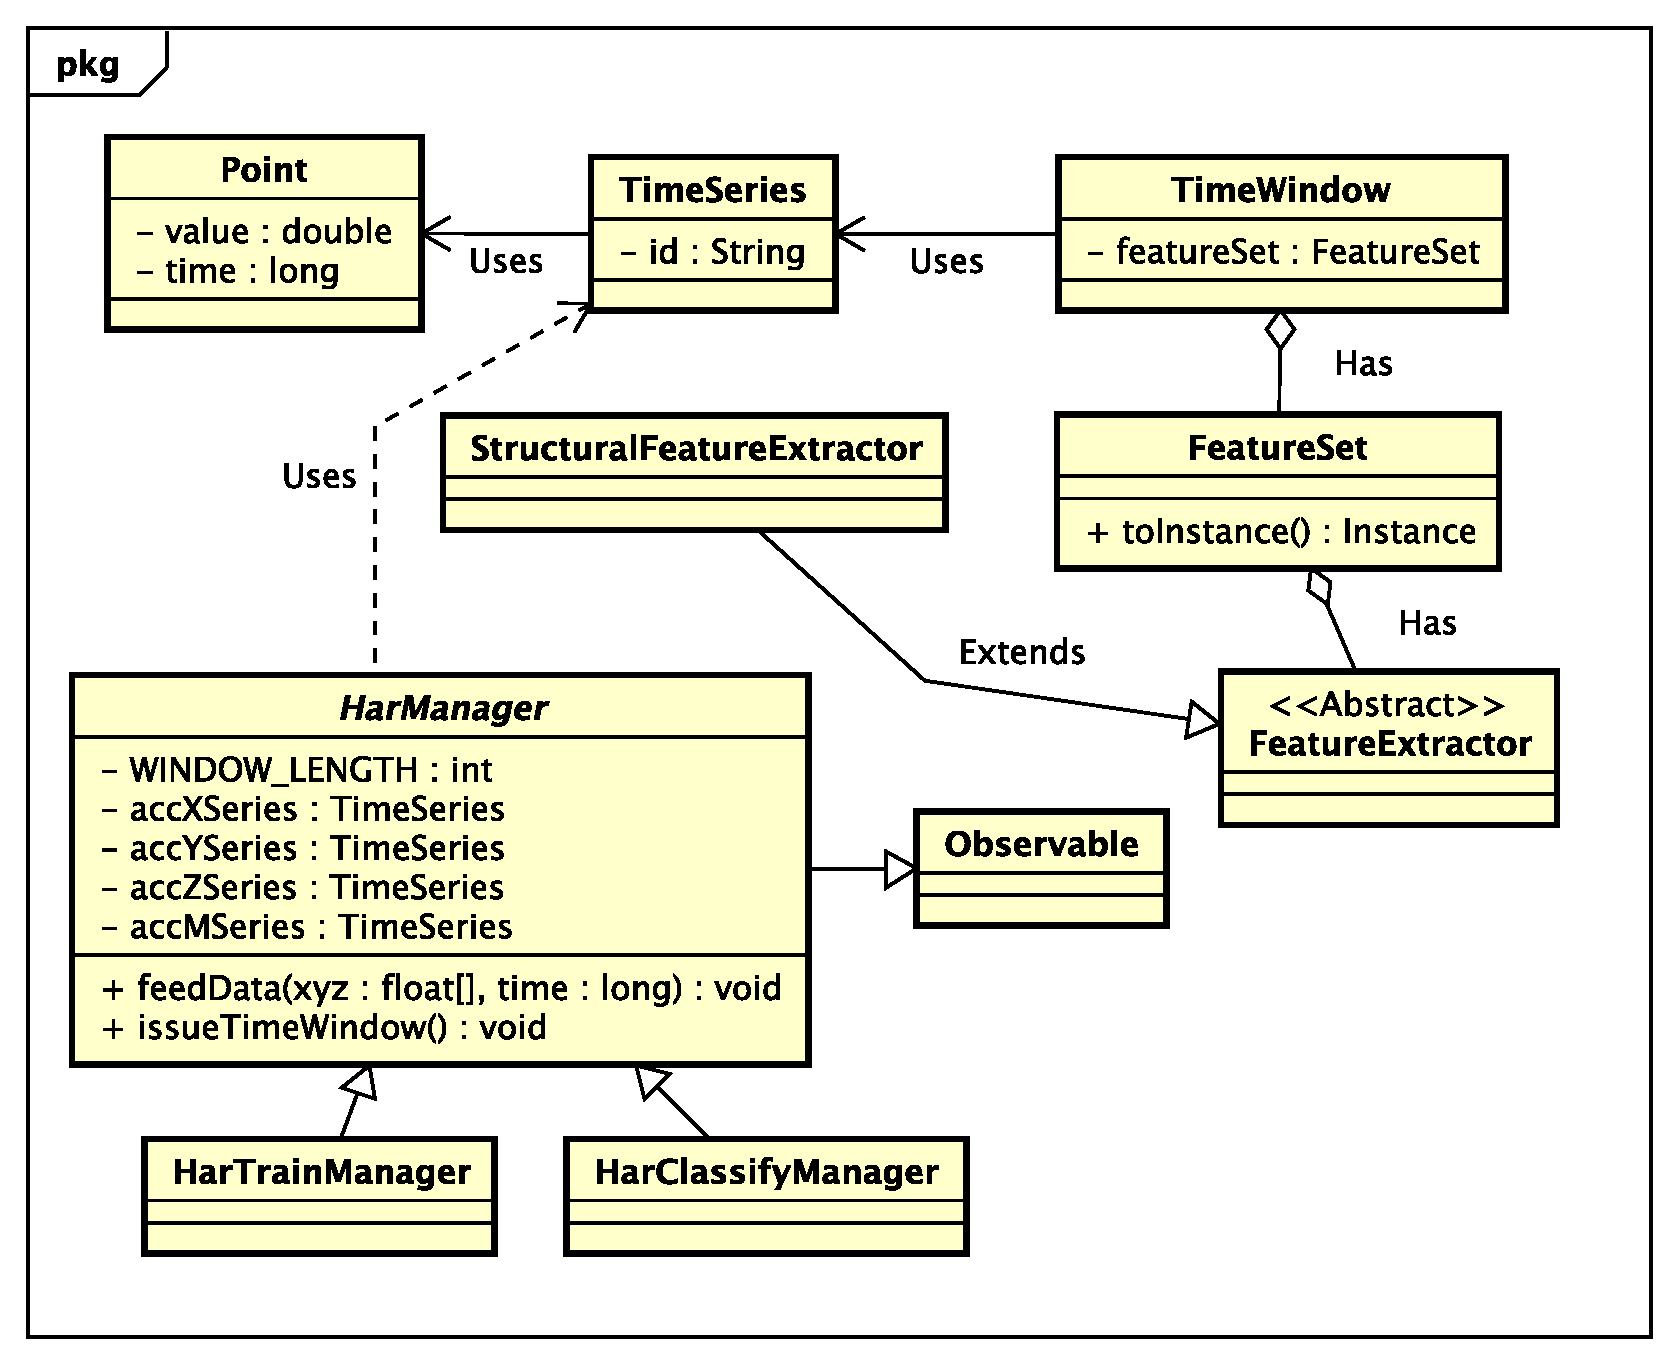
\includegraphics[width=13cm]{har_system_class_diagram_pdf}
        \caption{HAR system class diagram (simplified)}
        \label{fig:har_system_impl_class_diagram}
    \end{figure}
    
    Class \textbf{Point} is responsible for storing the readings of the smartphone accelerometer sensor. Every instance of the class stores the accelerometer readings such as the amount of acceleration in X, Y and Z direction in a class variable \textit{value} as well as a \textit{time} class variable which is used to compare different instances of the class.
        
    \textbf{TimeSeries} class extends \textit{ArrayList} which is one of the widely used data structure in the Java language since it allows easy storing and manipulation of list of items \citep{oraclearrayList_2017}. TimeSeries class stores a list of \textit{Point} values labeled by an \textit{id} value (see figure \ref{fig:har_system_impl_class_diagram}). For example, to store the accelerometer \textit{X} direction acceleration values in a TimeSeries instance, its \textit{id} could store value such as "accX".
        
    \textbf{TimeWindow} class extends Hashtable. That allows for storing values accessed by key \citep{oraclehashtable_2017}. For example, TimeWindow class provides means of storing \textit{TimeSeries} objects and accessing them via key. The key value used to associate every TimeSeries object is the same as the \textit{id} value of the TimeSeries object itself.
        
        
\section{Self-Management System}

\section{"Active Minutes" application}   
    
    \subsection{Realm Database}
    
    \subsection{Data collection service}
    
    \subsection{Active Minutes service}
    
    \subsection{Application UI}  




    
    
    
    